% ======================================================== %
% Przeczytaj plik amuthesis-doc.pdf, aby poznać opcje      %
% klasy `amuthesis`                                        %
% ======================================================== %
\documentclass[oneside,polski,logo]{amuthesis}

% Zdefiniuj kodowanie pliku źródłowego (domyślnie utf8)
\usepackage[utf8]{inputenc}

% ======================================================== %
% Dane autora i pracy                                      %
% ======================================================== %

% --- Autor pracy
\author{Kamil Tyrek, Mateusz Hypś, Jakub Kozubal}
% --- Numer albumu
\album{434797, 434699, 434726}
% --- Tytuł pracy (w języku polskim i angielskim)
\titlePL{Projekt i implementacja gry „The Lore: Story of the fallen warrior”}
\titleEN{Project and implementation of game „The Lore: Story of the fallen warrior”}
% --- Typ pracy (inżynierska, licencjacka, magisterska)
\type{inżynierska}
\graphicspath{ {./images} }
% --- Wydział (wykaz skrótów):
% --- --- WA    --- Wydział Anglistyki
% --- --- WB    --- Wydział Biologii
% --- --- WCh   --- Wydział Chemii
% --- --- WFPiK --- Wydział Filologii Polskiej i Klasycznej
% --- --- WF    --- Wydział Fizyki
% --- --- WH    --- Wydział Historyczny
% --- --- WMiI  --- Wydział Matematyki i Informatyki
% --- --- WNGiG --- Wydział Nauk Geograficznych i Geologicznych
% --- --- WNPiD --- Wydział Nauk Politycznych i Dziennikarstwa
% --- --- WNS   --- Wydział Nauk Społecznych
% --- --- WN    --- Wydział Neofilologii
% --- --- WPAK  --- Wydział Pedagogiczno-Artystyczny w Kaliszu
% --- --- WPiA  --- Wydział Prawa i Administracji
% --- --- WSE   --- Wydział Studiów Edukacyjnych
% --- --- WT    --- Wydział Teologiczny
% --- --- IKE   --- Instytut Kultury Europejskiej w Gnieźnie
\faculty{WMiI}
% --- Kierunek (w mianowniku)
\field{informatyka}
% --- Specjalność (w formie mianownikowej)
% --- (ustaw puste, jeśli bez specjalności)
% --- Promotor (w dopełniaczu)
\supervisor{dr Bartłomieja Przybylskiego}
% --- Data złożenia pracy (Miasto, miesiąc rok)
\date{Poznań, styczeń 2021}

% --- Płeć autora (M/K)
\stsex{M}
% --- Zgoda na udostępnienie pracy w czytelni (TAK/NIE)
\stread{TAK}
% --- Zgoda na udostępnienie pracy w zakresie ochrony (TAK/NIE)
\stprotect{TAK}
% --- Data podpisania oświadczenia (Miasto, data)
\stdate{Poznań, \today{} r.}

% ======================================================== %
% Dodatkowe pakiety wykorzystywane w pracy                 %
% ======================================================== %

\usepackage{lipsum}

% ======================================================== %
% Zasadnicza część dokumentu                               %
% ======================================================== %

\begin{document}

% Strona tytułowa
\maketitle
% Oświadczenie
\makestatement
% Spis treści
\tableofcontents

% ======================================================== %
% Właściwa część pracy                                     %
% ======================================================== %

\chapter{Wstęp}
\section{Cel i założenia projektu}
Celem projektu jest stworzenie gry platformowej, zawierającej elementy zręcznościowe oraz łamigłówki. Głównym założeniem projektu jest gra, która zaciekawi swoją fabułą oraz trudnością. Wstępnie prosty zamysł samouczka, w większości gier jest raczej elementem wprowadzającym do rozgrywki, która powinna robić się trudniejsza w im dalszym etapie rozgrywki się znajdujemy, w przypadku naszej gry jest odwrócony. Samouczek poza wprowadzaniu poszczególnych elementów rozgrywki, którymi jest między innymi przedstawienie sterowania oraz funkcjonalności i wstępnych mechanik jest również wymagający, od gracza zależy jakie umiejętności w trakcie rozgrywki będzie rozwijać, aby przejście kolejnych poziomów było łatwiejsze (z perspektywy gracza). Dużą wagę w projekcie przywiązujemy do mini-gier, które występują w trakcie przechodzenia poszczególnych poziomów. Występują dwa rodzaje mini-gier: opcjonalne (te które przejść możemy w celu sprawdzenia siebie oraz zdobycia punktów doświadczenia) oraz wymagane, które trzeba przejść, aby znaleźć się w dalszym etapie gry. Użytkownik posiada do dyspozycji punkty doświadczenia, drzewko umiejętności oraz ekwipunek. Punkty doświadczenia możemy wydawać bezpośrednio w drzewku umiejętności, w którym zadaniem gracza jest wybranie odpowiednich umiejętności zależnie od tego jaką strategię rozgrywki chce przyjąć. Warto pamiętać jednak, że im głębiej będziemy rozwijać daną gałęź tym umiejętności będą bardziej pomocne co sprawia, że gracz musi zastanowić się dobrze nad decyzjami dotyczącymi rozwijania konkretnych umiejętności w drzewku. Ekwipunek służy do zdobywania przedmiotów potrzebnych w trakcie rozgrywki m.in. do otwierania drzwi czy rozpoczęcia opcjonalnej mini-gry. W projekcie są wykorzystane 2 style tworzenia poziomów: ortographic i perspective. Wszystkie animacje w projekcie są tworzone z użyciem technologii inverse kinematics co pozwala na stałe dodawanie nowych animacji i poprawianie już istniejących.
\section{Organizacja pracy}
Charakter projektu sprawił, iż nie można w naszym zespole jasno podzielić typów zadań, które realizujemy w ramach projektu. Wynikiem tego jest to, iż nowe funkcjonalności są realizowane zazwyczaj przez jedną osobę od początku do końca, nie ma podziału, podobnego jak w przypadku aplikacji z frontendem i backendem.


Jako metodykę pracy przyjęto Scrum. Głównymi powodami tej decyzji jest doświadczenie części zespołu w tej metodyce oraz przejrzystość i rozsądne zarządzanie pracą. Nie rozważano innych metodyk pracy. Przy zarządzaniu pracą wspomaga nas serwis JIRA, który pozwala zarządzać regularne sprinty – w pierwszym semestrze dwutygodniowe, w drugim semestrze tygodniowe. 


Kod źródłowy zarządzany jest poprzez GitHub. Dla przejrzystości pracy, każdy commit na GitHub oznaczany jest id zadania na Jirze, dzięki czemu wchodząc w zadanie widzimy commit powiązany z jego rozwiązaniem. W momencie rozpoczęcia zadania deweloper, jeśli następuje potrzeba, tworzy podzadania do zadań na Jirze. Dotyczy to większych zadań, których wykonanie polega na tworzeniu większej ilości funkcjonalności. Dzięki temu realizując nowe zadania, o podobnej budowie, można sugerować się podobnym sposobem działania zadania. Po każdym commicie programista wyznacza ile czasu poświęcił na zadanie, poprzez wbudowaną w Jirze funkcjonalność “Log Work”. Gdy zadanie zostanie zakończone, programista oznacza je statusem “DONE”.  


Z racji wybranej metodyki, dokonano również przydzielenia odpowiednich ról członkom zespołu. Podział ról wygląda następująco:

\begin{itemize}
	\item Kamil Tyrek - Development Team, Scrum Master
	\item Jakub Kozubal -Development Team, Product Owner
	\item Mateusz Hypś - Development Team
\end{itemize}

\section{Podział prac}
\subsection{Kamil Tyrek - tworzenie elementów logicznych i ich algorytmika}
W tym rozdziale zostaną przedstawione sposoby tworzenia elementów logicznych. Część z przedstawionych łamigłówek została użyta w projekcie końcowym. Przykładem są tutaj przesuwane puzzle - rozgrywka polegająca na przesunięciu elementu, celem ułożenia poprawnego obrazka. Algorytmika stojąca za losowaniem kolejności elementów nie jest trywialna, ponieważ źle wylosowana kolejność puzzli powoduje, iż mogą być niemożliwe do ułożenia.

Zostanie przedstawiona też logika mini-gry z ustawieniem odpowiednich ruch, celem połączenia dwóch końców rur. Podobnie jak w poprzednim przykładzie, do rozwiązania tej zagadki potrzebna jest odpowiednia liczba rur danego typu - pionowe, poziome, skrętne. 

Następnym przykładem będzie logika stojąca za rozgrywką, która nie jest dostępna w końcowym projekcje, a chodzi tutaj o generowanie labiryntu. Nietrywialnym problemem jest wygenerowanie takiej planszy, aby możliwe było przejście z punktu A do punktu B. W tym rozdziale postaramy się przedstawić rozwiązanie tego problemu, przy użyciu odpowiednich algorytmów.

\subsection{Mateusz Hypś - Zarządzanie projektem gry komputerowej z wykorzystaniem Agile}
W rozdziale zostanie opisany proces zarządzania projektem z wykorzystaniem metodyki zwinnej. Omówione i porównane zostaną podejścia Agile i Agile Game Development oraz zastosowania tych metodyk, w porównaniu z innymi stosowanymi w praktyce. Przedstawione zostaną najważniejszych idee stojące za metodykami Agile m.in. framework SCRUM. Następnie omówione zostanie zastosowanie tych metodyk w projekcie “The Lore”, z uwzględnieniem problemów w trakcie realizacji tego projektu. 
\subsection{Jakub Kozubal}
W tym rozdziale zostaną przedstawione sposoby tworzenia poruszania się postaci. Zaznaczone zostaną główne różnice między fizyką rzeczywistą, a tą stosowaną w grach jak i przedstawienie wielu sposobów rozwiązania tej samej funkcjonalności. Ponadto przedstawiony zostanie proces tworzenia postaci. Do tego pojawi się też opisanie problemów takich jak sterowanie postaci w powietrzu oraz oddziaływanie sił z otoczenia (m.in. poruszające się platformy). Zostanie także przedstawione i przeanalizowane działanie każdej umiejętności występującej w drzewku odpowiedzialnej za poruszanie się.

\section{Użyta technologia - Unity}
 W naszym projekcie postanowiliśmy wybrać UNITY jako środowisko do stworzenia naszej gry. Wynikało to z możliwości jakie oferuje oraz z jakości i czytelności, stworzonej przez twórców, oficjalnej dokumentacji. Pozwala nam na tworzenie gier dwuwymiarowych czy trójwymiarowych oraz interaktywnych materiałów, na przykład animacje czy wizualizacje. W razie problemów możemy również wykorzystywać oficjalne forum na którym rzesza użytkowników dzieli się swoimi wskazówkami a także oficjalny sklep – Asset Store, w którym możemy wykupić materiały potrzebne do naszej gry. UNITY działa na każdym systemie operacyjnym, tj. Windows, macOS oraz Linux. Gwarantuje nam również możliwość stworzenia aplikacji nie tylko na komputery osobiste, ale także przeglądarki internetowe, konsole gier wideo oraz urządzenia mobilne. Dzięki aktualizacji silnika do wersji 5.1.1 ta lista wzrasta do 22 platform sprzętowych, w tym gogle wirtualnej rzeczywistości takie jak Oculus Rift.
W przeszłości można było tworzyć aplikacje w trzech językach:
\begin{itemize}
	\item UnityScript (swego rodzaju pochodna JavaScript’u)
	\item C\#
	\item Boo
\end{itemize}
Jednak wraz z piątą wersją silnika (wydaną w roku 2015) możliwość pisania w języku Boo została usunięta, pozostała tylko wsteczna kompatybilność w postaci możliwości kompilacji skryptów przez środowisko MonoDevelop. Podobny los dotknął UnityScript, którego wsparcie zakończyło się na wersji 2018.2 (najnowsza wersja stabilna to 2019.3.4). Z tych względów nasz wybór musiał paść na język C\#, w którym zostały napisane wszystkie nasze skrypty. Jako jedyny jest wciąż wspierany przez autorów, co zaowocowało drastycznym wzrostem popularności wśród użytkowników.

\chapter{Zarządzanie projektem gry komputerowej z wykorzystaniem Agile}
\section{Zarządzanie projektem informatycznym}
\subsection{Proces zarządzania projektem i jego geneza}
\subsection{Cykl życia projektu informatycznego}
\subsection{Metody pomocne w zarządzaniu projektami informatycznymi}
\subsection{Ryzyko oraz powody niepowodzeń  projektów informatycznych}

\section{Zarządzanie projektem gry komputerowej - The Lore}
\subsection{Proces planowania projektu}
\subsection{Wykorzystane systemy i metody projektowe}
\subsection{Rola i wpływ kierownika projektu} 
\subsection{Cykl życia projektu The Lore}

\chapter{Zagadki logiczne}
\section{Przesuwane puzzle}
\subsection{Omówienie zagadnienia i ogólne założenia}
Przesuwane puzzle to układanka, złożona zazwyczaj z kwadratowej liczby elementów, najczęściej jest to szesnaście pól. Pola są jednakowych rozmiarów i oznaczone są liczbami od 1 do (n-1), gdzie n to liczba dostępnych pól w układance. Jedno pole jest puste, pozwala to na przeniesienie sąsiednich elementów puzzli względem siebie. Rozgrywka kończy się, gdy ułożymy puzzle w odpowiedniej kolejności, według rosnącego porządku liczb lub powstania odpowiedniego obrazka. Trudno określić kto odpowiada za stworzenie zagadaki. Wiadomym jest, że w 1878 roku pochodzący ze Stanów Zjednoczonych Samuel Loyd wypromował układankę, jednak prawdopodobnie nie jest to jego pomysł. Dość popularną nazwą na rozgrywkę jest "piętnastka", określającą ilość dostępnych pól w najpopularniejszym ułożeniu - 4x4.  

W grze The Lore gracze staną przez rozwiązaniem zagadki gdzie do dyspozycji mamy dziewięć pól. Podczas projektowania układanki w grze uznano, iż zagadka może być dość trudna, a korzyści płynące z rozwiązania jej będą nieadekwatne do straconego czasu, stąd ilość pól jest mniejsza niż w najpopularniejszej wersji rozgrywki.
\subsection{Algorytmika}
\subsubsection{Pojedynczy element puzzle - PuzzleBlock}

Każdy pojedynczy element puzzla jest zainicjalizowany jako obiekt, który określamy jako PuzzleBlock. Obiekt posiada koordynaty, które określają jego położenie w przestrzeni na układance.

\begin{figure}[h]
	\centering
	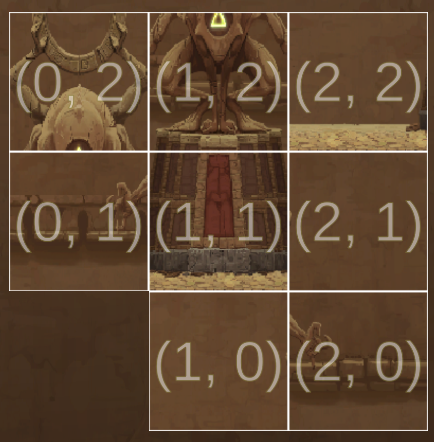
\includegraphics[width=6cm]{images/tyrek/coord_puzzle.png}
	\caption{Koordynaty każdego pola. Przykład z gry The Lore}
\end{figure}

Tak jak na załączonym przykładzie, wartość x rośnie w prawą stronę, zaś Y w górę, gdzie x dotyczy położenia w poziomie, a y w pionie. W założeniach przedstawiona została logika, która mówiła, iż element może zostać przemieszczony wtedy i tylko wtedy, gdy pole obok niego jest wolne, czyli nie posiada żadnego PuzzleBlock - elementu z liczbą lub obrazkiem. Dla lepszego efektu wizualnego, w grze The Lore element porusza się stopniowo, aby sprawiał wrażenie, iż porusza się realistycznie. Z racji, iż w Unity każda akcja wykonuje się podczas pokazywania kolejnej klatki, element porusza się w minimalnym stopniu przez sekundę. 
(TODO: tu można jakoś opisać, o ile jest sens - nie wpływa to na algorytmikę)

\subsubsection{Plansza - Puzzle. Losowanie kolejności puzzli}
Plansza rozgrywki posiada 8 elementów PuzzleBlock oraz jedno puste pole.  Algorytm powinien wylosować dla 8 pól ich położenie na planszy - tak jak w wyżej przedstawionym przykładzie. W tym celu na początku losujemy dla każdego bloku wartość od 0 do 8. W C\# możemy to zrobić przy użyciu funkcji  System.Random().Next(a, b). Przykładowo:
\begin{lstlisting}[
language={[Sharp]C},
rulecolor=\color{blue!80!black},
caption={Fragment klasy \texttt{Puzzle.cs}}
]
private int randomPosition()
{
    int pos = 0;
    do
    {
        pos = new System.Random().Next(0, 9);
    }
    while (isOnBoard[pos]);
    isOnBoard[pos] = true;
    return pos;
}
\end{lstlisting}

Gdzie isOnBoard[pos] jest tablicą, która weryfikuje, czy dane pole nie jest już zajęte. Jeśli jest, ponownie losujemy wartość dla PuzzleBlock. Oczywiście to nie koniec - z tej wartości musimy stworzyć położenie w postaci (x, y), gdzie x to położenie w poziomie, a y w pionie. W tym celu jedna z tych wartości będzie resztą dzielenia wylosowanej pozycji przez trzy (ilość pól w linii), a druga ilorazem całkowitym pozycji i liczby trzy. 

\subsection{Przedstawienie przykładu w grze The Lore}

\section{Zagadka z rurami}
\subsection{Omówienie zagadnienia}
\subsection{Algorytmika}
\subsection{Przedstawienie przykładu w grze}

\section{Zagadka z otwieraniem skrzyni}
\subsection{Omówienie zagadnienia}
\subsection{Algorytmika}

\section{Labirynt}
\subsection{Omówienie zagadnienia}
\subsection{Algorytmika}
\subsection{Przykłady użycia}

\end{document}
